\documentclass[4paper]{article}
\usepackage[spanish]{babel}
%\usepackage[ansinew]{inputenc}
\usepackage[utf8x]{inputenc}
%\usepackage[utf-8]{inputenc}
%\usepackage[T1]{fontenc}
\usepackage{graphicx}
\usepackage{multicol}
\usepackage{hyperref}
\usepackage{float}
%\usepackage{longtable}
%\usepackage{array}
%\usepackage{multirow}
%\usepackage[latin1]{inputenc}
%\inputencoding{latin}
\newcommand{\J}{JavaScript}
\newcommand{\s}{express}
\newcommand{\M}{mysql}
\newcommand{\R}{REST}
\newcommand{\N}{node.js}




%\newcommand{\j}{JavaScript }

\renewcommand{\tablename}{Tabla}
\author{Manuel Molino Milla}
\title{\textbf{Servicio \R ~ con \N ~ y \s }}
\date{\today}

\begin{document}
\maketitle 
\tableofcontents
\newpage

\section{Persistencia}
Como persistencia usaremos SGBD \M
\subsection{Introducción \M}
\begin{itemize}
\item Es un sistema de gestión de bases de datos relacional desarrollado bajo licencia dual GPL/Licencia comercial por Oracle Corporation 
\item Está considerada como la base datos open source más popular del mundo.
\item MySQL fue inicialmente desarrollado por MySQL AB (empresa fundada por David Axmark, Allan Larsson y Michael Widenius). 
\item MySQL A.B. fue adquirida por Sun Microsystems en 2008
\item Ésta a su vez fue comprada por Oracle Corporation en 2010.
\item En 2009 se creó un fork denominado MariaDB por algunos desarrolladores (incluido algunos desarrolladores originales de MySQL) descontentos con el modelo de desarrollo y el hecho de que una misma empresa controle a la vez los productos MySQL y Oracle Database.
\item  Tradicionalmente se considera uno de los cuatro componentes de la pila de desarrollo LAMP y WAMP.
\item MySQL es usado por muchos sitios web grandes y populares, como Wikipedia, Google, Facebook, Twitter, Flickr  y YouTube.
\item MySQL es muy utilizado en aplicaciones web, como Joomla, Wordpress, Drupal o phpBB,
\end{itemize}

\subsection{Características \M}
\begin{itemize}
\item Está desarrollado en su mayor parte en ANSI C y C++
\item MySQL es una base de datos muy rápida en la lectura cuando utiliza el motor no transaccional MyISAM.
\item Amplio subconjunto del lenguaje SQL.
\item Disponibilidad en gran cantidad de plataformas y sistemas.
\item Posibilidad de selección de mecanismos de almacenamiento que ofrecen diferentes velocidades de operación, soporte físico, capacidad, distribución geográfica, transacciones...
\item Transacciones y claves foráneas.
\item Conectividad segura.
\item Replicación.
\item Búsqueda e indexación de campos de texto.
\item Permite escoger entre múltiples motores de almacenamiento para cada tabla (MyISAM, InnoDB, Memory/heap, \dots)
\item Un sistema de reserva de memoria muy rápido basado en threads
\item Un sistema de privilegios y contraseñas que es muy flexible y seguro, y que permite verficación basada en el host.
\item Funciona en diferentes plataformas.
\end{itemize}

\subsection{Soporte transaccional \M}
\begin{itemize}
\item Incluyen un soporte completo de ACID (atómica, consistente, aislada, duradera)
\item Bloqueo a nivel de filas
\item Soporte de transacciones con múltiples versiones donde los lectores no bloquean a los escritores y viceversa.
\item 
\end{itemize}

\subsection{Instalación \M}
En sistemas Ubuntu
\begin{quote}
sudo apt-get install mysql-server
\end{quote}
En sistemas windows, simplemente descargar el instalador y ejecutarlo.

\subsection{Tutorial \M}
\href{http://www.tutorialesprogramacionya.com/mysqlya/}{Tutorial mysql}

\newpage

\subsection{Tipo de datos en \M}
\begin{itemize}
\item Numéricos.
\item Fecha.
\item String.
\end{itemize}
\textbf{TIPO NUMÉRICOS:}
\begin{description}
\item[INT (INTEGER)] Ocupación de 4 bytes con valores entre -2147483648 y 2147483647 o entre 0 y 4294967295.
\item[SMALLINT] Ocupación de 2 bytes con valores entre -32768 y 32767 o entre 0 y 65535.
\item[TINYINT] Ocupación de 1 bytes con valores entre -128 y 127 o entre 0 y 255.
\item[MEDIUMINT] Ocupación de 3 bytes con valores entre -8388608 y 8388607 o entre 0 y 16777215.
\item[BIGINT] Ocupación de 8 bytes con valores entre -8388608 y 8388607 o entre 0 y 16777215.
\item[DECIMAL (NUMERIC)] Almacena los números de coma flotante como cadenas o string.
\item[FLOAT (m,d)] Almacena números de coma flotante, donde \emph{m} es el número de dígitos de la parte entera y \emph{d} el número de decimales.
\item[DOUBLE (REAL)] Almacena número de coma flotante con precisión doble. Igual que FLOAT, la diferencia es el rango de valores posibles.
\item[BIT (BOOL, BOOLEAN)] Número entero con valor 0 o 1.
\end{description}
\textbf{TIPO FECHA:}
\begin{description}
\item[DATE] Válido para almacenar una fecha con año, mes y día, su rango oscila entre  \emph{1000-01-01} y \emph{9999-12-31}.
\item[DATETIME] Almacena una fecha (año-mes-día) y una hora (horas-minutos-segundos), su rango oscila entre  \emph{1000-01-01 00:00:00} y \emph{9999-12-31 23:59:59}.
 \item[TIME] Válido para almacenar una hora (horas-minutos-segundos). Su rango de horas oscila entre -838-59-59 y 838-59-59. El formato almacenado es \emph{HH:MM:SS}.
\item[TIMESTAMP] Almacena una fecha y hora UTC. El rango de valores oscila entre \emph{1970-01-01 00:00:01} y 2\emph{038-01-19 03:14:07}.
\item[YEAR] Almacena un año dado con 2 o 4 dígitos de longitud, por defecto son 4. El rango de valores oscila entre 1901 y 2155 con 4 dígitos. Mientras que con 2 dígitos el rango es desde 1970 a 2069  (70-69).
\end{description}
\textbf{TIPO STRING:}
\begin{description}
\item[CHAR] Ocupación fija cuya longitud comprende de 1 a 255 caracteres.
\item[VARCHAR] Ocupación variable cuya longitud comprende de 1 a 255 caracteres.
\item[TINYBLOB] Una longitud máxima de 255 caracteres. Válido para objetos binarios como son un fichero de texto, imágenes, ficheros de audio o vídeo. No distingue entre minúculas y mayúsculas.
\item[BLOB] Una longitud máxima de 65.535 caracteres. Válido para objetos binarios como son un fichero de texto, imágenes, ficheros de audio o vídeo. No distingue entre minúculas y mayúsculas.
\item[MEDIUMBLOB] Una longitud máxima de 16.777.215 caracteres. Válido para objetos binarios como son un fichero de texto, imágenes, ficheros de audio o vídeo. No distingue entre minúculas y mayúsculas.
\item[LONGBLOB] Una longitud máxima de 4.294.967.298 caracteres. Válido para objetos binarios como son un fichero de texto, imágenes, ficheros de audio o vídeo. No distingue entre minúculas y mayúsculas.
\item[SET] Almacena 0, uno o varios valores una lista con un máximo de 64 posibles valores.
\item[ENUM] Igual que SET pero solo puede almacenar un valor.
\item[TINYTEXT] Una longitud máxima de 255 caracteres. Sirve para almecenar texto plano sin formato. Distingue entre minúculas y mayúsculas.
\item[TEXT] Una longitud máxima de 65.535 caracteres. Sirve para almecenar texto plano sin formato. Distingue entre minúculas y mayúsculas.
\item[MEDIUMTEXT] Una longitud máxima de 16.777.215 caracteres. Sirve para almecenar texto plano sin formato. Distingue entre minúculas y mayúsculas.
\item[LONGTEXT] Una longitud máxima de 4.294.967.298 caracteres. Sirve para almecenar texto plano sin formato. Distingue entre minúculas y mayúsculas.
\end{description}

\newpage

\subsection{Creación de base de datos y usuarios}
\begin{quote}
CREATE DATABASE nombre\_baseDatos
\end{quote}
Para utilizar en el cliente \emph{\M}
\begin{quote}
use nombre\_baseDatos
\end{quote}
Podemos saber las tablas que contiene
\begin{quote}
show tables;
\end{quote}
En cuanto a la creación de usuarios:
\begin{verbatim}
GRANT ALL PRIVILEGES ON dbTest.* To 'user'@'hostname' IDENTIFIED BY 'password';
\end{verbatim}
Otra forma de hacerlo es
\begin{verbatim}
CREATE USER 'new_user'@'localhost' IDENTIFIED BY 'new_password';
GRANT ALL ON my_db.* TO 'new_user'@'localhost';
\end{verbatim}
Los permisos pueden ser
\begin{figure}[H]
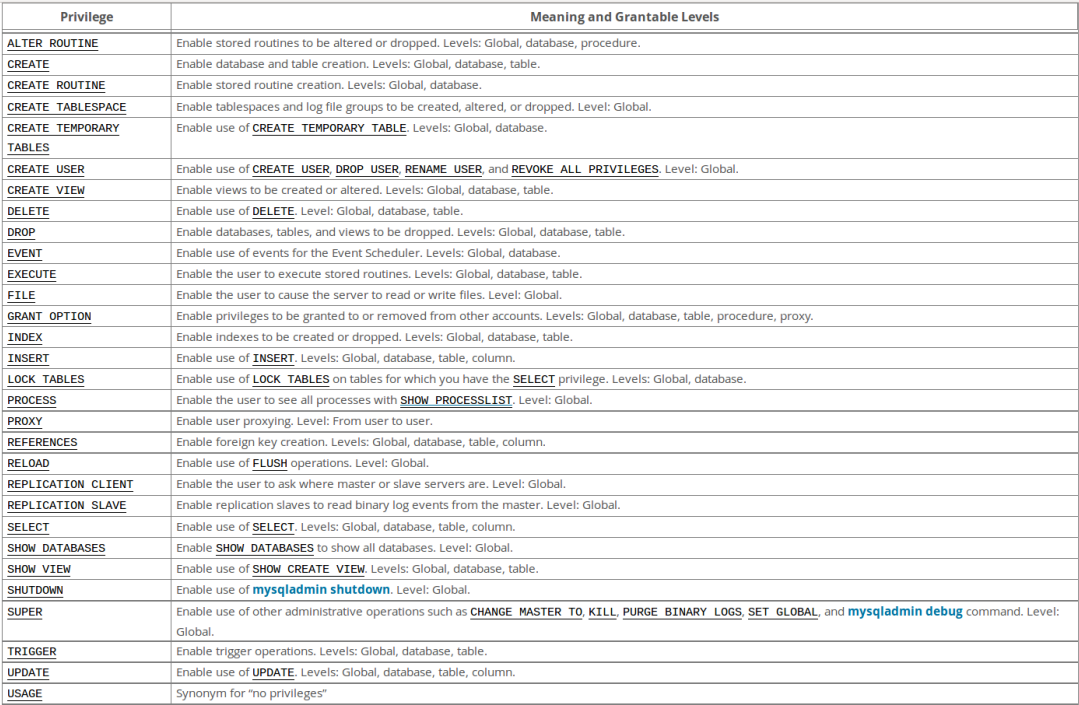
\includegraphics[scale=0.5]{../imagenes/mysql.png}
\end{figure}
Cada vez que se actualiza o cambiamos permisos,hay que refrescar los privilegios mediante \emph{FLUSH PRIVILEGES;}.\\
\newpage
Podemos conocer los usuarios en \M
\begin{quote}
select User from mysql.user;
\end{quote}
Si deseamos saber qué usuarios tienen alguna clase de acceso a cada base de datos, es posible cruzar las tablas user y db con la siguiente consulta SQL:
\begin{verbatim}
 select u.User,d.Db from mysql.user u,mysql.db d where u.User=d.User;
\end{verbatim}
Podemos conocer los permisos que tiene con:
\begin{quote}
SHOW GRANTS FOR jordi@localhost;
\end{quote}
\subsection{Ejemplo de creación de tablas en \M}
\begin{verbatim}
CREATE TABLE IF NOT EXISTS equipment (
    equip_id int(5) NOT NULL AUTO_INCREMENT,
    type varchar(50) DEFAULT NULL,
    install_date DATE DEFAULT NULL,
    color varchar(20) DEFAULT NULL,
    working bool DEFAULT NULL,
    location varchar(250) DEFAULT NULL,
    PRIMARY KEY(equip_id)
    ); ENGINE=InnoDB DEFAULT CHARSET=latin1;
\end{verbatim}

\subsection{Ejercicio}
Crear una base de datos denominada \emph{prueba} que contenga una tabla llamada \emph{libros}, que tenga como campos un \emph{id} autoincrementable, el \emph{autor} y \emph{título} del libro, mas el \emph{precio} del mismo. Como \emph{engine} usamos \emph{InnoDB} y \emph{charset utf8}.\\
El titulo debe ser único en la tabla\\
Creamos un usuario denominado prueba 
\subsection{Funciones en \M}
\begin{itemize}
\item Una función en MySQL es una rutina creada para tomar unos parámetros, procesarlos y retornar en un salida.
\item Se diferencian de los procedimientos en las siguientes características:
\begin{itemize}
\item Solamente pueden tener parámetros de entrada IN y no parámetros de salida OUT o INOUT
\item Deben retornar en un valor con algún tipo de dato definido
\item Solo retornan un valor individual, no un conjunto de registros.
\end{itemize}
\end{itemize}
¿Cómo se crea una función?
\begin{quote}
CREATE FUNCTION nombre\_función (parametro1,parametro2,...)
RETURNS tipoDato
[atributos de la rutina]
bloque de instruccciones
\end{quote}
La única diferencia entre la creación de un procedimiento y una función es que la sintaxis de una función contiene la palabra reservada RETURNS para indicar que tipo de dato se retornará.\\
Ejemplo:
\begin{verbatim}
DELIMITER $$
CREATE FUNCTION hello_world()
  RETURNS TEXT
  LANGUAGE SQL
BEGIN
  RETURN 'Hello World';
END;
$$
DELIMITER ;
\end{verbatim}
Ejecutamos:
\begin{quote}
SELECT hello\_world();
\end{quote}
Mas completo:
\begin{verbatim}
DROP FUNCTION IF EXISTS hello_world;
DELIMITER $$
CREATE FUNCTION hello_world(addressee TEXT)
  RETURNS TEXT
  LANGUAGE SQL -- This element is optional and will be omitted from subsequent examples
BEGIN
  RETURN CONCAT('Hello ', addressee);
END;
$$
DELIMITER ;
\end{verbatim}
Ejecutamos con:
\begin{quote}
SELECT hello\_world('Earth');
\end{quote}

\newpage

\subsection{Procedimiento en \M}
\begin{itemize}
\item Un procedimiento es un conjunto de instrucciones que se guardan en el servidor para un posterior uso, ya que se ejecutarán frecuentemente.
\item Se nombra con la clausa \emph{PROCEDURE}
\item A diferencia de las funciones, los procedimientos son rutinas que no retornan en ningún tipo de valor.
\item Simplemente se llaman desde el cliente con un comando y las instrucciones dentro del procedimiento se ejecutarán.
\item Son seguros pues ocultan el nombre de las tablas a usuarios que no tengan los privilegios para manipular datos.
\item Simplemente llaman los procedimientos sin conocer la estructura de la base de datos.
\end{itemize}
Creación de un procedimiento ren \M
\begin{verbatim}
CREATE PROCEDURE nombre ([parámetro1,parámetro2,...])
[Atributos de la rutina]
BEGIN instrucciones
END
\end{verbatim}
Un procedimiento puede tener uno o mas parámetros o también no tener ninguno. Puede carecer de atributos o puede poseer varios. Y el cuerpo del procedimiento es un bloque de instrucciones definido.
\begin{itemize}
\item Un parámetro es un dato necesario para el funcionamiento del procedimiento.
\item Los parámetros pueden ser de entrada (IN), salida (OUT) o entrada/salida (INOUT) y deben tener definido un tipo.
\item Un parámetro de entrada en un dato que debe ser introducido en la llamada del procedimiento para definir alguna acción del bloque de instrucciones.
\item Para especificar el tipo de parámetro seguimos la siguiente sintaxis:
\end{itemize}
\begin{quote}
[\{IN$|$OUT$|$INOUT\}] nombre TipoDeDato
\end{quote}
\newpage
Ejemplo de de procedimiento:
\begin{verbatim}
DELIMITER //

CREATE PROCEDURE numeros_1_hasta_n (IN n INT)
BEGIN
DECLARE contador INT DEFAULT 1;
WHILE contador<=n DO
SELECT contador;
SET contador = contador + 1 ;
END WHILE;
END//

DELIMITER ;
\end{verbatim}
¿Cómo se ejecuta?
\begin{quote}
CALL numeros\_1\_hasta\_n(5)
\end{quote}
Otro ejemplo: procedimiento que inserta un cliente en la base de datos.
\begin{verbatim}
DELIMITER //
CREATE PROCEDURE insertar(id_cliente INT,
        nombre_cliente VARCHAR(100), apellido_cliente VARCHAR(100))
COMMENT 'Procedimiento que inserta un cliente a la base de datos'
BEGIN
IF NOT EXISTS ( SELECT C.ID 
FROM CLIENTE AS C 
WHERE C.ID = id_cliente) THEN
INSERT INTO CLIENTE(ID, NOMBRE, APELLIDO)
VALUES ( id_cliente,nombre_cliente,apellido_cliente);
ELSE
SELECT 'Este cliente ya existe en la base de datos!';
END IF;
END//

DELIMITER ;
\end{verbatim}

\subsection{Ejercicio}
\begin{itemize}
\item Crea una función que dado el id de un libro de la tabla libros de la BD anterior, nos devuelva el precio de venta al público con el IVA incluido (21\%)
\item Crea un procedimiento que nos sirva bien para actualizar o bien para añadir un nuevo libro, dependiendo si existe o no el libro.
\end{itemize}

\section{Proyecto}
Se quiere realizar una aplicación \R ~ eb \N ~ para gestionar los pedidos de la empresa. Como SGBD usaremos \M ~ y las especificaciones son:
\begin{itemize}
\item Caracterizaremos el nombre de los clientes con el nombre de la empresa y su email.
\item En los pedidos hay que hacer constar la fecha.
\item Los pedidos constaran de productos así como la cantidad de cada uno de ellos.
\item Los productos tienen un precio estipulado y pertenecen a una categoría determinada.
\item La categoría de los productos se conoce con el nombre de la misma.
\item Acompañaremos de una función que nos calcule el precio total de un producto.
\end{itemize}
Se pide:
\begin{itemize}
\item Diagram ER de la base de datos.
\item La estructura de las correspondientes tablas. Las aportamos en un script de tipo sql.
\item El API REST con las funciones CRUD típicas sobre clientes, pedido, producto, categoría, \dots
\item El desarrollo de la aplicación usando \N
\end{itemize}

\newpage

\section{express-generator}
Permite crear un proyecto con \emph{\N} ~y \emph{express} usando el patrón \emph{MVC}\\
Lo instalamos de la siguiente manera:
\begin{quote}
 npm install express-generator -g
\end{quote}
Gneremao un proyecto con:
\begin{quote}
express app
\end{quote}
Que genera la siguiente salida:
\begin{verbatim}
  warning: the default view engine will not be jade in future releases
  warning: use `--view=jade' or `--help' for additional options


   create : app
   create : app/package.json
   create : app/app.js
   create : app/public
   create : app/public/stylesheets
   create : app/public/stylesheets/style.css
   create : app/routes
   create : app/routes/index.js
   create : app/routes/users.js
   create : app/views
   create : app/views/index.jade
   create : app/views/layout.jade
   create : app/views/error.jade
   create : app/bin
   create : app/bin/www

   install dependencies:
     $ cd app && npm install

   run the app:
     $ DEBUG=app:* npm start

   create : app/public/javascripts
   create : app/public/images

\end{verbatim}
\newpage
Creando la siguiente estructura de directorios:
\begin{figure}[H]
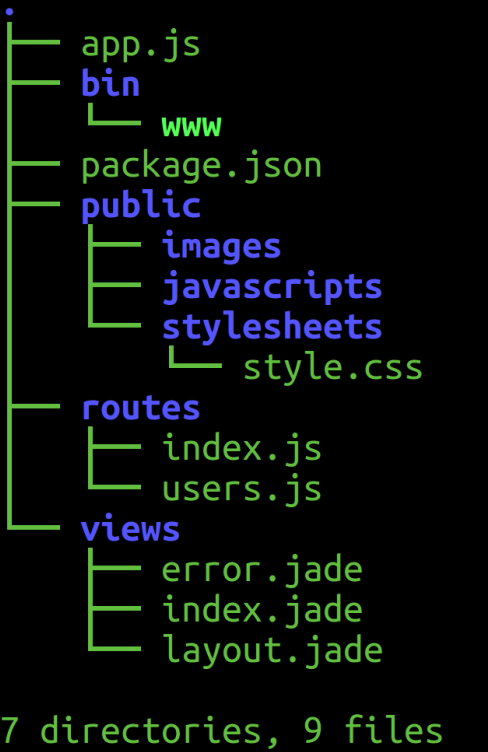
\includegraphics[scale=0.8]{../imagenes/tree.png}
\end{figure}
\newpage
El fichero package.json contiene la estructura del proyecto, con nombre, dependencias, \dots
\begin{verbatim}
{
  "name": "app",
  "version": "0.0.0",
  "private": true,
  "scripts": {
    "start": "node ./bin/www"
  },
  "dependencies": {
    "body-parser": "~1.15.2",
    "cookie-parser": "~1.4.3",
    "debug": "~2.2.0",
    "express": "~4.14.0",
    "jade": "~1.11.0",
    "morgan": "~1.7.0",
    "serve-favicon": "~2.3.0"
  }
}
\end{verbatim}
Debemos configurar la aplicación con\emph{ npm install}, que se encarga de instalar las dependencias. El fichero \emph{bin/www} se encarga de crear el servidor. Y lo iniciamos con \emph{npm start}
%1\subsection{MVC}
%Para configurar correctamente el patrón MVC debemos realizar los siguientes pasos:
%\begin{itemize}
%\item Creamos una carpeta denominada application en la carpeta raíz de la application.
%\item Creamos en dicha carpeta application las subcarpetas denominadas \emph{models} y \emph{controllers}.
%\item Movemos las carpetas \emph{vistas(views)} y \emph{rutas(routes)} a la carpeta \emph{application}
%\item Realizamos los siguientes cambios en \emph{app.js}:
%\begin{verbatim}
%app.set('views', path.join(__dirname, 'views'));
%POR
%app.set('views', path.join(__dirname, 'application', 'views'));
%también cambiamos
%var routes = require('./routes/index'); 
%var users = require('./routes/users'); 
%POR
%var routes = require('./application/routes/index'); 
%var users = require('./application/routes/users'); 
%\end{verbatim}
%\item En /application/routes/index.js cambiamos:
%\begin{verbatim}
%/* GET home page. */ 
%router.get('/', function(req, res, next) { 
%  res.render('index', { title: 'Express' }); 
%});
%POR
%var ctrlMain = require('../controllers/main'); 
%/* GET home page. */ 
%router.get('/', ctrlMain.index);
%\end{verbatim}
%\item Creamos el fichero \emph{/application/controllers/main.js} con el siguiente contenido:
%\begin{verbatim}
%/* GET home page */ 
%module.exports.index = function(req, res){ 
%  res.render('index', { title: 'Express' }); 
%}; 
%\end{verbatim}
%\item Reiniciamos el proyecto.
%\end{itemize}
\end{document}